\documentclass{article}
\usepackage[utf8]{inputenc}
\usepackage{mathtools, nccmath}
\usepackage{mathabx}
\usepackage{mathrsfs}
\usepackage{natbib}
\usepackage{graphicx}
\usepackage{cancel}
\usepackage{upquote}
\usepackage{pgfplots}
\usepackage{amssymb}
\pgfplotsset{width=10cm,compat=1.9}
\usepgfplotslibrary{external}
\tikzexternalize
\usepackage{hyperref}
\usepackage{xparse}
\usetikzlibrary{through}

\usepackage{tikz}
\usetikzlibrary{angles,quotes}

\newcommand{\handC}{\mathscr{C}}

\title{Mate 1: Curs \#1}
\author{Profesor: Radu Gologan}
\date{1 Octombrie 2019}

\DeclarePairedDelimiterX{\set}[1]{\{}{\}}{\setargs{#1}}
\NewDocumentCommand{\setargs}{>{\SplitArgument{1}{;}}m}
{\setargsaux#1}
\NewDocumentCommand{\setargsaux}{mm}
{\IfNoValueTF{#2}{#1} {#1\,\delimsize|\,\mathopen{}#2}}%{#1\:;\:#2}

\begin{document}
    
    \maketitle
    \section{Multimi}
        Definim o \textbf{multime} $A$ formata din elemente distincte ce au o proprietate prin notatia: $A = \set{x;x\ are\ proprietatea\ \textit{P}}$ \\
        Definim relatia de \textbf{incluziune}: $\subseteq$ pe doua multimi A si B astfel:\\
        $A \subseteq B \iff (\forall a \in A \implies a \in B)$\\
        Definim urmatoarele operatii:
        \begin{itemize}
            \item \textbf{reuniune}: $A \cup B = \set{x; x \in A\ sau\ x\in B}$
            \item \textbf{intersectie}: $A \cap B = \set{x; x \in A\ si\ x\in B}$
            \item \textbf{diferenta}: $A \setminus B = \set{x; x \in A\ si\ x\notin B}$
            \item \textbf{complementara}: $B \subseteq A \iff C^B_A = A \setminus B$
        \end{itemize}
        Definim \textbf{produs cartezian} intre doua multimi A si B astfel:\\
        $A\times B = \set{(a, b); a \in A\ si\ b\in B}$\\ \\
        Fie $I$ o familie de indici(multime) si $A_i,\ i\in I$ o familie de multimi indexate de $I$.
        Definim urmatoarele operatii:
        \begin{itemize}
            \item \textbf{Reuniunea tuturor multimilor}: $\displaystyle{\bigcup_{i\in I}} A_i = \set{a; \exists i \in I, a \in A_i}$
            \item \textbf{Intersectia tuturor multimilor}: $\displaystyle{\bigcap_{i\in I}} A_i = \set{a; \forall i \in I, a \in A_i}$
        \end{itemize}
        Exemplu: $\displaystyle{\bigcup_{x\in\mathbb{R}}}\set{x}=\mathbb{R}$
    \section{Relatii}
        Definim o \textbf{relatie} pe o multime X o submultime $R \subseteq X \times X$:\\
        $R = \set{(x,y); x\in X\ si\ y \in X}$\\
        Vom nota $(x,y) \in R \iff xRy$\\
        Definim o \textbf{relatie de echivalenta} pe $X$, o relatie $R$ cu urmatoarele proprietati:
        \begin{itemize}
            \item \textbf{reflexivate}: $xRx, \forall x \in X$
            \item \textbf{simetrie}: $xRy \implies yRx,\ \forall (x,y) \in R$
            \item \textbf{tranzitivitate}: $xRy\ si\ yRz \implies xRz,\ \forall (x,y),(y,z) \in R$
        \end{itemize}
        Exemple:
        \begin{itemize}
            \item Relatia de egalitate
            \item Relatia de echivalenta a figurilor geometrice
            \item Fie $n \in \mathbb{N}^*$, introducem pe $\mathbb{Z}$ relatia:\\ $m,p \in \mathbb{Z},\ m\equiv p (mod\ n) \iff n | (m-p)$\\
            Pentru $i = \overline{0,n-1}$, definim \textbf{clasa de resturi a lui $i$}: $\hat{i} = \set{i+n\cdot k; k \in \mathbb{Z}}$ si \textbf{multimea
                claselor de resturi modulo $n$}: $\mathbb{Z}_n = \set{\hat{0},\hat{1},...,\widehat{n-1}}$
        \end{itemize}
        In general, pentru $(X,R)$ o relatie de echivalenta, vom nota:\\ $\forall x \in X, \hat{x} = \set{y;yRx}\implies X = \displaystyle{\bigcup_{x\in X}}\hat{x}\ si\ x \cancel{R}y \implies \hat{x} \cap \hat{y} = \emptyset$\\
        vom nota \textbf{multimea claselor de echivalenta} sau \textbf{spatiul cat} $\set{\hat{x}}_{x\in X} = X/_R$.\\ 
        Exemple:
        \begin{itemize}
            \item Fie $\Delta = \set{(x,y); x,y \in [0,1]}$ suprafata unui patrat si $\rho$ o relatie de echivalenta astfel incat:\\
            Daca $M=(x_1,y_1)\ cu\ x_1\in (0,1)\ si\ y_1 \in [0,1]\ si\ N=(x_2,y_2)\ cu\ x_2\in (0,1)\ si\ y_2 \in [0,1]\implies M\rho N \iff M = N$\\
            Daca $M=(x_1,y_1)\ cu\ x_1\in \{0,1\}\ si\ y_1 \in [0,1]\ si\ N=(x_2,y_2)\ cu\ x_2\in \{0,1\}\ si\ y_2 \in [0,1]\implies M\rho N \iff y_1=y_2$
            \begin{center}
                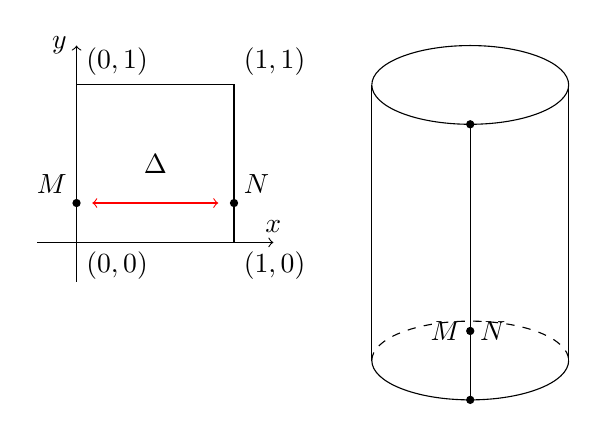
\begin{tikzpicture}
                      \draw (0,0) -- (0,2) -- (2,2) -- (2,0) -- cycle;
                      \draw[->] (0,-.5) -- (0,2.5) node[left] {$y$};
                      \draw[->] (-.5,0) -- (2.5,0) node[above] {$x$};
                      \draw (0,0) node[anchor=north west] {$(0,0)$};
                      \draw (0,2) node[anchor=south west] {$(0,1)$};
                      \draw (2,0) node[anchor=north west] {$(1,0)$};
                      \draw (2,2) node[anchor=south west] {$(1,1)$};
                      \draw (0,0.5) node[anchor = south east] {$M$};
                      \draw (2,0.5) node[anchor = south west] {$N$};
                      \draw (1,1) node {$\Delta$};
                      \fill (0,0.5) circle[radius=1.5pt];
                      \fill (2,0.5) circle[radius=1.5pt];
                      \draw[<->,red] (0.2,0.5) -- (1.8,0.5);
                      
                      \draw (5,2) ellipse (1.25 and 0.5);
                      \draw (3.75,2) -- (3.75,-1.5);
                      \draw (3.75,-1.5) arc (180:360:1.25 and 0.5);
                      \draw [dashed] (3.75,-1.5) arc (180:360:1.25 and -0.5);
                      \draw (6.25,-1.5) -- (6.25,2);  
                      \fill (5,1.5) circle[radius=1.5pt];
                      \fill (5,-2) circle[radius=1.5pt];
                      \draw (5,1.5) -- (5,-2);
                      \fill (5,-1.125) circle[radius=1.5pt];
                      \draw (5,-1.125) node[anchor=west] {$N$};
                      \draw (5,-1.125) node[anchor=east] {$M$};
                  \end{tikzpicture}
            \end{center}
            Se observa din constructie ca $\Delta/_\rho =\ suprafata\ laterala\ a\ unui\ cilindru$
        
            \item Fie $\Delta = \set{(x,y); x,y \in [0,1]}$ suprafata unui patrat si $\rho$ o relatie de echivalenta astfel incat:\\
            Daca $M=(x_1,y_1)\ cu\ x_1\in (0,1)\ si\ y_1 \in [0,1]\ si\ N=(x_2,y_2)\ cu\ x_2\in (0,1)\ si\ y_2 \in [0,1]\implies M\rho N \iff M = N$\\
            Daca $M=(x_1,y_1)\ cu\ x_1\in \{0,1\}\ si\ y_1 \in [0,1]\ si\ N=(x_2,y_2)\ cu\ x_2\in \{0,1\}\ si\ y_2 \in [0,1]\implies M\rho N \iff y_1= 1 - y_2$
            \begin{center}
                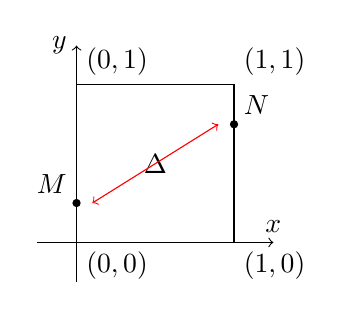
\begin{tikzpicture}
                      \draw (0,0) -- (0,2) -- (2,2) -- (2,0) -- cycle;
                      \draw[->] (0,-.5) -- (0,2.5) node[left] {$y$};
                      \draw[->] (-.5,0) -- (2.5,0) node[above] {$x$};
                      \draw (0,0) node[anchor=north west] {$(0,0)$};
                      \draw (0,2) node[anchor=south west] {$(0,1)$};
                      \draw (2,0) node[anchor=north west] {$(1,0)$};
                      \draw (2,2) node[anchor=south west] {$(1,1)$};
                      \draw (0,0.5) node[anchor = south east] {$M$};
                      \draw (2,1.5) node[anchor = south west] {$N$};
                      \draw (1,1) node {$\Delta$};
                      \fill (0,0.5) circle[radius=1.5pt];
                      \fill (2,1.5) circle[radius=1.5pt];
                      \draw[<->,red] (0.2,0.5) -- (1.8,1.5);
                  \end{tikzpicture}
                  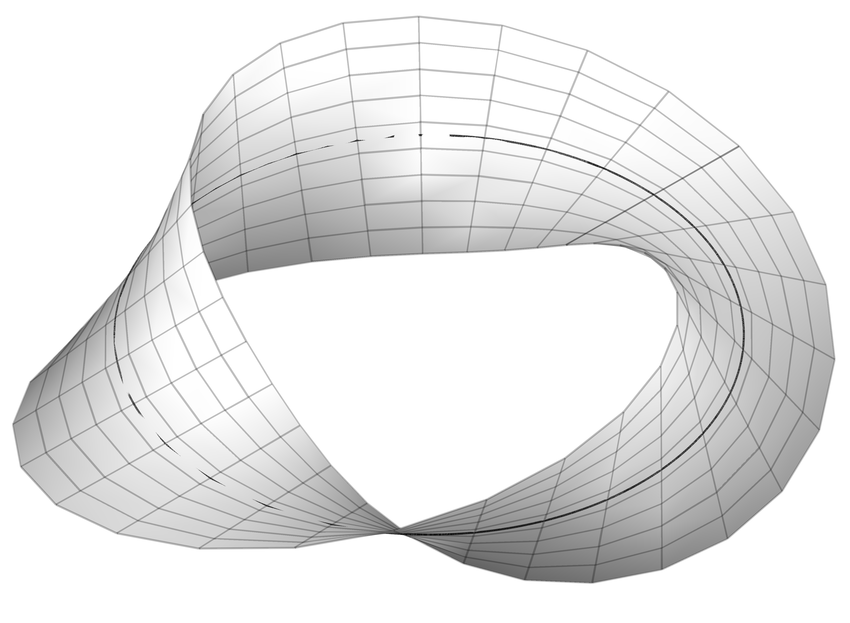
\includegraphics[width=4cm, height=3cm]{MobiusStrip.png}
            \end{center}
            Se observa din constructie ca $\Delta/_\rho =\ suprafata\ definita\ de\ o\ banda\ Mobius$
            
            \item Fie $\Delta = \set{(x,y); x,y \in [0,1]}$ suprafata unui patrat si $\rho$ o relatie de echivalenta astfel incat:\\
            Daca $M=(x_1,y_1)\ cu\ x_1\in (0,1)\ si\ y_1 \in (0,1)\ si\ N=(x_2,y_2)\ cu\ x_2\in (0,1)\ si\ y_2 \in (0,1)\implies M\rho N \iff M = N$\\
            Daca $M=(x_1,y_1)\ cu\ x_1\in \{0,1\}\ si\ y_1 \in [0,1]\ si\ N=(x_2,y_2)\ cu\ x_2\in \{0,1\}\ si\ y_2 \in [0,1]\implies M\rho N \iff y_1= 1 - y_2$\\
            Daca $M=(x_1,y_1)\ cu\ x_1\in [0,1]\ si\ y_1 \in \{0,1\}\ si\ N=(x_2,y_2)\ cu\ x_2\in [0,1]\ si\ y_2 \in \{0,1\}\implies M\rho N \iff x_1= x_2$
            \begin{center}
                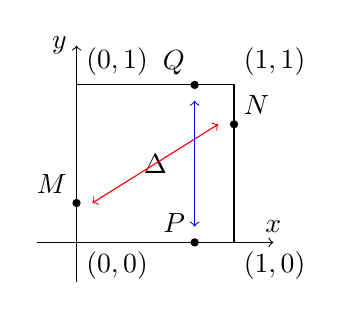
\begin{tikzpicture}
                      \draw (0,0) -- (0,2) -- (2,2) -- (2,0) -- cycle;
                      \draw[->] (0,-.5) -- (0,2.5) node[left] {$y$};
                      \draw[->] (-.5,0) -- (2.5,0) node[above] {$x$};
                      \draw (0,0) node [anchor=north west] {$(0,0)$};
                      \draw (0,2) node[anchor=south west] {$(0,1)$};
                      \draw (2,0) node[anchor=north west] {$(1,0)$};
                      \draw (2,2) node[anchor=south west] {$(1,1)$};
                      \draw (0,0.5) node[anchor = south east] {$M$};
                      \draw (2,1.5) node[anchor = south west] {$N$};
                      \draw (1.5,0) node[anchor = south east] {$P$};
                      \draw (1.5,2) node[anchor = south east] {$Q$};
                      \draw (1,1) node {$\Delta$};
                      \fill (0,0.5) circle[radius=1.5pt];
                      \fill (2,1.5) circle[radius=1.5pt];
                      \fill (1.5,0) circle[radius=1.5pt];
                      \fill (1.5,2) circle[radius=1.5pt];
                      \draw[<->,red] (0.2,0.5) -- (1.8,1.5);
                      \draw[<->,blue] (1.5,0.2) -- (1.5,1.8);
                  \end{tikzpicture}
                  
\includegraphics[width=3cm, height=4cm]{KleinBottle.png}
            \end{center}
            Se observa din constructie ca $\Delta/_\rho =\ suprafata\ definita\ de\ o\ sticla\ Klein$
        
        \end{itemize}
        
    \section{Relatii de ordine}
        $(X,R)$ o relatie pe $X$ se numeste \textbf{relatie de ordine} daca si numai daca are urmatoarele proprietati:
        \begin{itemize}
            \item Reflexivitate
            \item \textbf{Antisimetrie:} $xRy\ si\ yRx \implies x=y$
            \item Tranzitivitate
        \end{itemize}
        O relatie de ordine se numeste \textbf{relatie de ordine totala} daca:\\ $\forall x,y \in X, xRy\ sau\ yRx$ \\
        O relatie de ordine se numeste \textbf{relatie de ordine partiala} daca nu este o relatie de ordine totala\\ \\
        Exemple:
        \begin{itemize}
            \item Notam $\mathscr{P}(X) = \set{A;A\subseteq X}, |X| = n \implies |\mathscr{P}(X)| = 2^n$ \textbf{multimea tuturor submultimilor lui X}\\
            $ARB \iff A \subseteq B$ este o relatie de ordine partiala.
        \end{itemize}
        De obicei, relatiile de ordine se noteaza $xRy \iff x \leq y$\\ \\
        Daca $(X,\leq)$ este o relatie de ordine si $A \subseteq X$, numim $M\in X$ \textbf{majorant pentru A} atunci cand $x \leq M,\ \forall x \in A$ si $m\in
        X$ \textbf{minorant pentru A} atunci cand $m \leq x,\ \forall x \in A$\\
        Definim $sup_A$ ca fiind cel mai mic majorant al multimii $A$, daca acesta exista, si $inf_A$ ca fiind cel mai mare minorant al multimii $A$, daca acesta exista.\\
        Explicitam:\\
        $sup_A = S \in X \iff x \leq S\ \forall x \in A\ si\ daca\ \forall S' \in X\ a.i.\ x \leq S' \implies S \leq S'$. Analog se defineste si $inf_A$.\\
        In $\mathbb{R},\ A \subseteq \mathbb{R},\ sup_A = S \in \mathbb{R} \iff a \leq S, \forall a \in A\ si\ \forall \epsilon > 0, \exists a \in A\ a.i.\
        S-\epsilon \leq a$.\\ \\
        Exercitiu:\\
        Fie $(a_n)_n,\ (b_n)_n$ doua siruri marginite in $\mathbb{R}$. Vom demonstra ca $sup(a_n+b_n) \leq sup(a_n) + sub(b_n)$.\\ \\
        Demonstratie:\\
        $a_i \leq sup(a_n),\forall i\ si\ b_i \leq sup(b_n),\forall i \implies a_i+b_i \leq sup(a_n) + sup(b_n),\forall i \implies sup(a_n+b_n) \leq sup(a_n) +
        sup(b_n)$
\end{document}

